\documentclass[border=2pt]{standalone}
\usepackage{amsmath}
\usepackage{tikz}
\usetikzlibrary{arrows.meta,calc,shapes.symbols}
\begin{document}
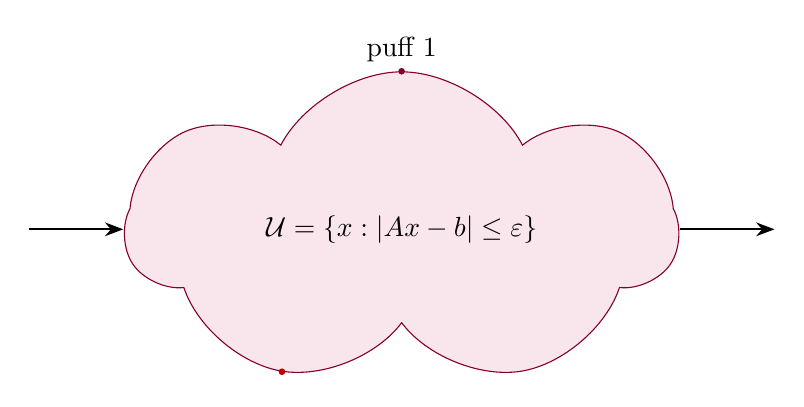
\begin{tikzpicture}[>=Stealth]
  \node[cloud,cloud puffs=7,cloud puff arc=125,aspect=2.2,
        draw=purple!70!black,fill=purple!10,minimum width=70mm,minimum height=40mm,
        inner sep=2mm] (set) {$\mathcal U=\{x:|Ax-b|\le\varepsilon\}$};
  \fill[purple!70!black] (set.puff 1) circle (1.2pt);
  \fill[red!75!black] (set.puff 4) circle (1.2pt);
  \draw[->,thick] ($(set.west)+(-12mm,0)$) -- (set.west);
  \draw[->,thick] (set.east) -- ++(12mm,0);
  \node[above] at (set.puff 1) {puff 1};
\end{tikzpicture}
\end{document}
